
\item A spring-block system is resting on a frictionless floor as shown in the figure. The spring constant is \(2.0 \, \text{N m}^{-1}\) and the mass of the block is \(2.0 \, \text{kg}\). Ignore the mass of the spring. Initially, the spring is in an unstretched condition. Another block of mass \(1.0 \, \text{kg}\) moving with a speed of \(2.0 \, \text{m s}^{-1}\) collides elastically with the first block. The collision is such that the \(2.0 \, \text{kg}\) block does not hit the wall. The distance, in \textit{metres}, between the two blocks when the spring returns to its unstretched position for the first time after the collision is \_\_\_\_\_.
\begin{center}
    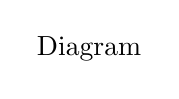
\begin{tikzpicture}
    \node {Diagram};
    \end{tikzpicture}
\end{center}
